\documentclass[letterpaper]{article}
\usepackage[margin=5mm]{geometry}
\usepackage{float}
\usepackage{subcaption}
\usepackage{booktabs}
\usepackage{multirow}
\usepackage{multicol}
\usepackage{graphicx}
\usepackage{paper_commands}

\begin{document}
\thispagestyle{empty} % Remove page number

\begin{figure}
    \centering
    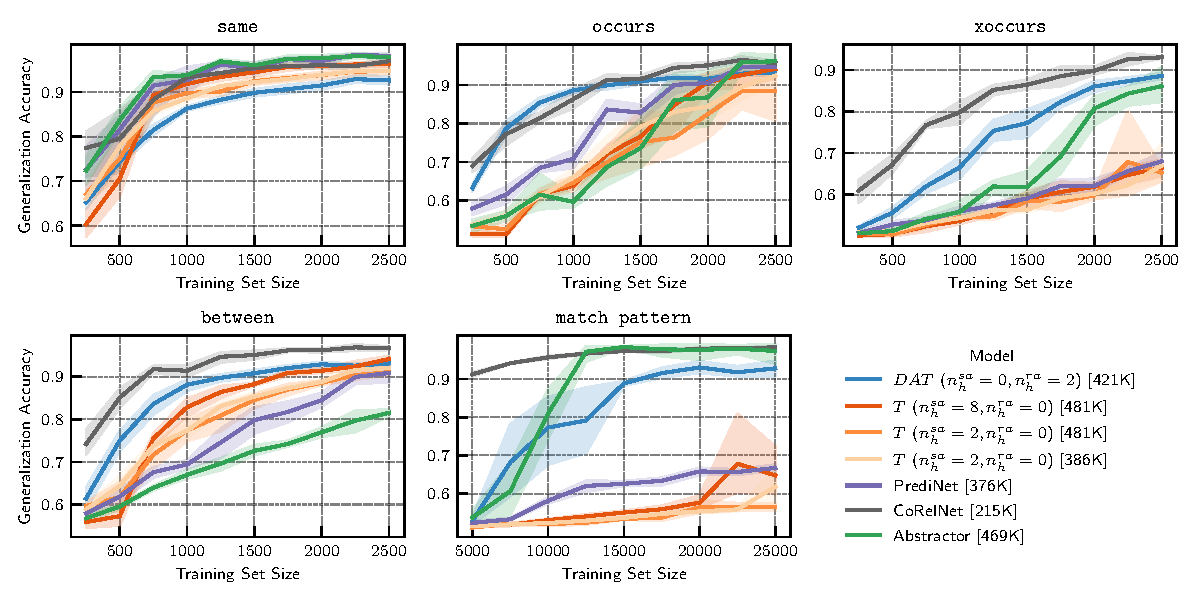
\includegraphics[width=0.8\textwidth]{figs/experiments/relgames/relgames_learning_curves_baseline_comparisons.pdf}
    % \caption{}
\end{figure}

\begin{figure}
    \centering
    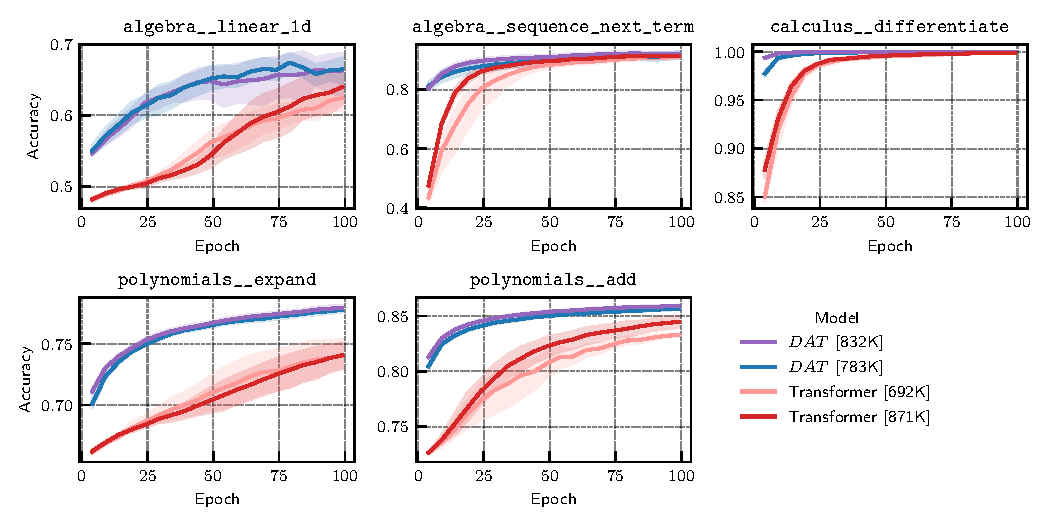
\includegraphics[width=0.8\textwidth]{figs/experiments/math/math_training_curves_interpolation.pdf}
    % \caption{}
\end{figure}


% \begin{figure}[ht]
%     \begin{subfigure}{0.44\textwidth}
%         \centering
%         \captionsetup{width=.9\linewidth}
%         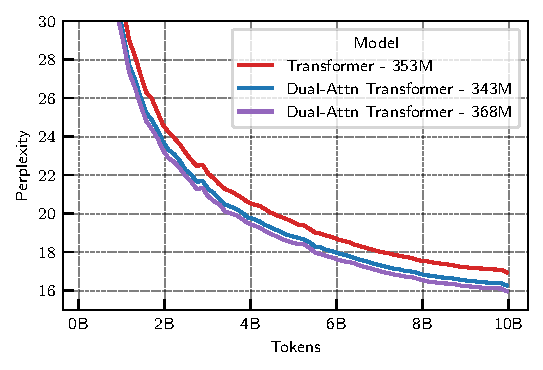
\includegraphics[width=\textwidth]{figs/experiments/fineweb/350M_scale_lm.pdf}
%         \caption{350M parameter scale ($\dmodel = 1024$, $\nlayers = 24$)}
%     \end{subfigure}
%     \begin{subfigure}{0.44\textwidth}
%         \centering
%         \captionsetup{width=.9\linewidth}
%         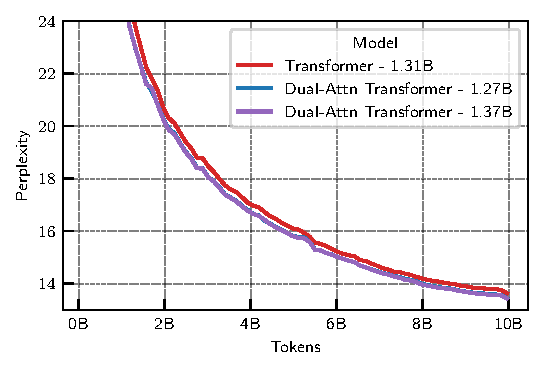
\includegraphics[width=\textwidth]{figs/experiments/fineweb/1_3B_scale_lm.pdf}
%         \caption{1.3B parameter scale ($\dmodel = 2048$, $\nlayers = 24$)}
%     \end{subfigure}
%     \caption{Perplexity curves on language modeling with the fineweb dataset. The $x$-axis indicates the number of tokens and the $y$-axis is the validation perplexity. \textit{DAT} learns faster and achieves smaller perplexity at multiple model size scales.}\label{fig:tiny_stories_val_loss_curves}
% \end{figure}

\begin{table}[]
    \centering
    \caption{Language Modeling on Fineweb dataset.}\label{tab:my-table}
    % \resizebox{\textwidth}{!}{%
    % \begin{tabular}{@{}l|ccccccc|c@{}}
    \begin{tabular}{@{}l|c|cccccc|c@{}}
    \toprule
    Model / Param count   & \# Tokens &$\dmodel$&$\nlayers$& $\nhsa$  & $\nhra$ & $n_r$ & $n_{kv}^{h}$ & Perplexity $\downarrow$ \\ \midrule\hline
    Transformer - 353M    & 10B       & 1024    & 24       & 16       & -        & -     & -           & 16.94     \\
    \textit{DAT} - 343M   & 10B       & 1024    & 24       & 8        & 8        & 32    & 4           & 16.26     \\
    \textit{DAT} - 368M   & 10B       & 1024    & 24       & 8        & 8        & 32    & 8           & 15.97     \\\midrule
    Transformer - 1.31B   & 10B       & 2048    & 24       & 32       & -        & -     & -           & 13.63     \\
    \textit{DAT} - 1.27B  & 10B       & 2048    & 24       & 16       & 16       & 64    & 8           & 13.44     \\
    \textit{DAT} - 1.37B  & 10B       & 2048    & 24       & 16       & 16       & 64    & 16          & 13.43     \\ \bottomrule
    % Model / Param count   &$\dmodel$&$\nlayers$& $\nhsa$  & $\nhra$ & $n_r$ & $n_{kv}^{h}$ & Perplexity $\downarrow$ \\ \midrule\hline
    % Transformer - 353M   & 1024    & 24       & 16       & -        & -     & -           & 16.944     \\
    % \textit{DAT} - 343M  & 1024    & 24       & 8        & 8        & 32    & 4           & 16.258     \\
    % \textit{DAT} - 368M  & 1024    & 24       & 8        & 8        & 32    & 8           & 15.969     \\\midrule
    % Transformer - 1.31B  & 2048    & 24       & 32       & -        & -     & -           & 13.630     \\
    % \textit{DAT} - 1.27B & 2048    & 24       & 16       & 16       & 64    & 8           & 13.440     \\
    % \textit{DAT} - 1.37B & 2048    & 24       & 16       & 16       & 64    & 16          & 13.426     \\ \bottomrule
    \end{tabular}%
    % }
    % & $n_s$ 
    % & -     
    % & 1024  
    % & 1024  
    % & -     
    % & 512   
    % & 2048  
\end{table}

\end{document}